
%%%  یک نمونه پروپوزال کارشناسی ارشد، نسخه 0.4
%%%  وحید دامن‌افشان، دانشگاه تبریز،       http://www.damanafshan.ir
%%%   آپدیت شده در تیرماه ۹۱
%توضیحات مربوط به هر بسته یا دستور را می‌توانید در خط بالای آن ببینید.

\documentclass[12pt,a4paper]{article}
%در ورژن جدید زی‌پرشین برای تایپ متن‌های ریاضی، این سه بسته، حتماً باید فراخوانی شود
\usepackage{amsthm,amssymb,amsmath}

%دستوری برای وارد کردن واژه‌نامه انگلیسی به فارسی
\newcommand\persiangloss[2]{#1\dotfill\lr{#2}\\}
%بسته‌ای برای تنطیم حاشیه‌های بالا، پایین، چپ و راست صفحه
%\usepackage[top=30mm, bottom=30mm, left=30mm, right=30mm]{geometry}
%بسته‌ای برای نمایش تصاویر قرار داده شده در متن
\usepackage{graphicx}
% بسته‌ و دستوراتی برای ایجاد لینک‌های رنگی با امکان جهش
\usepackage[pagebackref=false,colorlinks,linkcolor=blue,citecolor=magenta]{hyperref}
% چنانچه قصد پرینت گرفتن نوشته خود را دارید، خط بالا را غیرفعال و  از دستور زیر استفاده کنید چون در صورت استفاده از دستور زیر‌‌، 
% لینک‌ها به رنگ سیاه ظاهر خواهند شد و برای پرینت گرفتن، مناسب‌تر خواهد بود.
%\usepackage[pagebackref=false]{hyperref}
%بسته‌ای برای ظاهر شدن «مراجع»  در فهرست مطالب
\usepackage{tocbibind}
%فراخوانی بسته زی‌پرشین و دستورات مربوط به نوع فونت‌ها
\usepackage{xepersian}
%تغییرات نخ
\usepackage[bottom]{footmisc}
\usepackage{indentfirst}


\settextfont{B Nazanin}
% وارد کردن دستور بالا الزامی نیست؛ چون در صورت وارد نکردن آن، فونت پیش‌فرض به صورت خودکار، فراخوانی می‌شود.
% چنانچه می‌خواهید که اعداد داخل فرمول‌ها، فارسی باشد، دستور زیر را فعال کنید
%\setdigitfont{Times New Roman}


%%%%%%%%%%%%%%%%%%%%%%%%%%%%%%%%%%%%%%%%%%%%%%%%%%%
% تعریف قلم‌های فارسی و انگلیسی برای استفاده در بعضی از قسمت‌های متن
\defpersianfont\titr[Scale=1]{B Titr}
\defpersianfont\nastaliq[Scale=1.5]{IranNastaliq}
\defpersianfont\traffic[Scale=1]{B Traffic}
\defpersianfont\yekan[Scale=1]{B Yekan}
\DefaultMathsDigits
%اگر فونت‌های بالا را ندارید، دو خط بالا را غیر فعال و دو خط زیر را فعال کنید
%\defpersianfont\traffic[Scale=1]{XB Roya}
%\defpersianfont\yekan[Scale=1]{XB Kayhan}
%%%%%%%%%%%%%%%%%%%%%%%%%%%%%%%%%%%%%%%%%%%%%%%%%%%
% تعریف و نحوه ظاهر شدن قضایا، لم‌ها، تعریف‌ها و ...
\theoremstyle{definition}
\newtheorem{definition}{تعریف}[section]
\theoremstyle{theorem}
\newtheorem{theorem}[definition]{قضیه}
\newtheorem{lemma}[definition]{لم}
\newtheorem{proposition}[definition]{گزاره}
\newtheorem{corollary}[definition]{نتیجه}
\newtheorem{remark}[definition]{ملاحظه}
\theoremstyle{definition}
\newtheorem{example}[definition]{مثال}
%%%%%%%%%%%%%%%%%%%%%%%%%%%%%%%%%%%%%%%%%%%%%%%%%%%
\begin{document}
% دستوری جهت حذف کردن شماره صفحه و سربرگ، در صورت وجود (فقط در صفحه جاری)
\thispagestyle{empty}
\vspace*{-28mm}
% نحوه درج کردن لوگوی دانشگاه
\centerline{
\includegraphics[height=5cm]{logo.png}}
\begin{center}
%دستوری برای کم کردن فاصله بین لوگو و خط پایین آن
\vspace{-2mm}
{\large \titr
گروه مستقل مهندسی رباتیک
%دستوری برای تعیین فاصله بین دو خط
\\[2.1cm]
}

{\Large \titr
تمرین چهارم درس بینایی ماشین
\\[2cm]
استاد درس:
\\[.5cm]
دکتر صفابخش
\\[1.5cm]
\large 
تدریس‌یار: 
\\[0.5cm]
مهندس مجد
\\[1.5cm]
نام دانشجو:
\\[.5cm]
نوید خزاعی
\\[.5cm]
۹۲۱۳۵۰۰۸
\\[1.5cm]
}
%دستوری برای تعیین فاصله بین خطوط (نه دو خط) و تا وقتی که مقدار آن تغییر نکند، فاصله بین خطوط، همین مقدار است.
\baselineskip=1cm

{\large
خرداد ۱۳۹۳
}
\end{center}
%دستوری برای رفتن به صفحه جدید
\newpage
\baselineskip=1cm
%دستوری برای ظاهر شدن فهرست مطالب
\tableofcontents

\baselineskip=.75cm
\newpage 
\section{بخش اول}
%\cite{alvarez}
\subsection{{\lr {SIFT}}
}

\textbf{پرسش:}
 از کاربرد های الگوریتم \lr{SIFT} پیدا کردن تطابق بین تصاویر است. برای این کار کافی است الگوریتم \lr{SIFT} را بر روی هر دو تصویر اعمال کرده و سپس با استفاده از یک الگوریتم انطباق ویژگی میزان انطباق دو تصویر و یا محل وقوع یک تصویر در دیگری را تعیین کرد. با استفاده از الگوریتم \lr{SIFT} و یکی از روش‌های انطباق پیاده سازی شده در \lr{open-cv} مثل \lr{Brut-Force Matcher }، نقاط منطبق در دوجفت تصویر 10 (10-1 و 10-2) و 11(11-1 و 11-2) را بیابید. تصاویر را پیش از استفاده به تصاویر خاکستری تبدیل کنید.

\textbf{پاسخ:}
برای استفاده از الگوریتم \lr{SIFT} در \lr{OpenCV} دو روش وجود دارد. یکی استفاده از خود کلاس \lr{SIFT} است و دیگری استفاده از \lr{SiftFeatureDetector} و \lr{SiftDescriptorExtractor}. روال کار به این شکل است که باید ابتدا الگوریتم را بر روی هر تصویر اجرا نموده و نقاط کلیدی\LTRfootnote{ Key points} را استخراج کنیم و سپس هر کدام از نقاط را توسط یک بردارِ توصیف‌گر\LTRfootnote{ Descriptor vector} نمایش دهیم. در هر دو فاز از الگوریتم \lr{SIFT} استفاده می‌کنیم. سپس این بردارها را به یک سیستم تطبیق ویژگی\LTRfootnote{ Feature matching} می‌دهیم تا نقاط موجود در هر بردار را با دیگری تطبیق دهد. سپس بهترین تطبیق‌ها، که بر اساس فاصله از نقطه‌ی متناظر در بردار دیگر مشخص می‌شوند، انتخاب می‌شوند. در صورت وجود تطبیق‌های زیاد، می‌توان نتیجه گرفت که شی مورد نظر، در تصویر دوم نیز وجود دارد.

روش استفاده از \lr{SIFT} در این تمرین در زیر آورده شده‌است:‌
\begin{itemize}
\renewcommand{\labelitemi}{$\circ$}
\item 
با استفاده از کلاس \lr{SIFT} یک نمونه ایجاد می‌کنیم: 

\leftline{\lr{SIFT mysift(0, 3, 0.04, 10, 1);}}
که پارامترهای آن به ترتیب در زیر آورده شده‌است. مقادیر پیش‌فرض هر کدام نیز مشخص شده‌است:
\begin{itemize}
\renewcommand{\labelitemii}{$\bullet$}
\item 
\lr{int nfeatures = 0} : 
تعداد ویژگی‌هایی که در انتها باقی می‌مانند. انتخاب این تعداد بر اساس رتبه‌بندی خود الگوریتم در حین اجرا مخشص می‌شود.
\item 
\lr{int nOctaveLayers = 3} : 
تعداد لایه‌ها در هر اکتاو را مشخص می‌کند که در ایجاد هرم تصویر به‌کاربرده می‌شود. در الگوریتم اصلی\cite{sift} این تعداد به صورت پویا بر اساس رزولوشن تصویر محاسبه می‌شود.
\item 
\lr{double contrastThreshold = 0.04} : 
برای حذف ویژگی‌های ضعیف در نقاط با کنتراست کم استفاده می‌شود.
\item 
\lr{double edgeThreshold = 10} : 
حد آستانه‌ برای حذف ویژگی‌‌های گوشه‌مانند است. به این ترتیب که هر چقدر بیشتر باشد ویژگی‌های کمتری حذف می‌شوند. 
\item 
\lr{double sigma = 1.6} : 
واریانس فیلتر گاسی اعمال شده بر تصویر در اکتاو صفر را مشخص می‌کند. اگر تصویر با دوربین ضعیف گرفته‌شده است بهتر است این مقدار را کم کنیم. 

سپس برای استخراج نقاط کلیدی می‌توانیم از یک الگوریتم تطبیق‌دهنده‌ی ویژگی\LTRfootnote{ Feature matching} مانند \lr{FLANN} استفاده کنیم. پس از آن، تعدادی از بهترین تطبیق‌ها را انتخاب می‌کنیم و نقاط نظیر را به هم متصل می‌کنیم.

برای هر تصویر، نتیجه‌ی اجرا به همراه پارامترهای تنظیم شده آورده شده‌است: 
 
\end{itemize}
\end{itemize}

اجرا با پارامترهای پیش‌فرض:
\begin{center}
\makebox[\textwidth]{%
\begin{tabular}{@{}cc@{}}
\frame{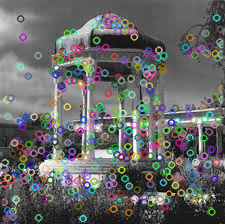
\includegraphics[height=60mm]{10-1-sift-src.png}} 
&
\frame{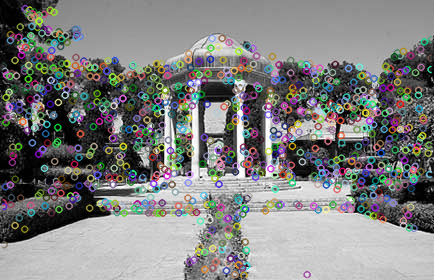
\includegraphics[height=60mm]{10-2-sift-cmp.png}}
\\ 
\small  \textbf{تصویر اصلی}  & \small \textbf{تصویر مقایسه}
\end{tabular}}
\end{center}

\begin{center}
\vspace{-0.5cm}
\makebox[\textwidth]{%
\begin{tabular}{@{}c}
\frame{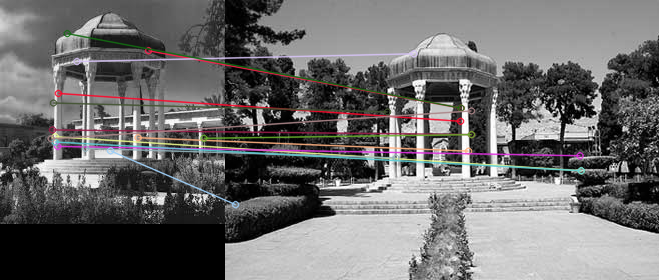
\includegraphics[height=60mm]{10-1-sift-match.png}} 
\\ 
\small  \textbf{نقاط منطبق با فاصله‌ی کمتر از ۱۰۰} 
\end{tabular}}
\vspace{-0.5cm}
\end{center}

اجرا با مقدار واریانس یک: 
\begin{center}
\vspace{-0.2cm}
\makebox[\textwidth]{%
\begin{tabular}{@{}cc@{}}
\frame{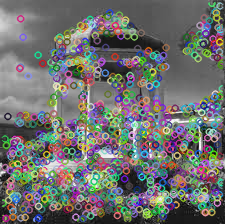
\includegraphics[height=55mm]{10-1-sift-src-1.png}} 
&
\frame{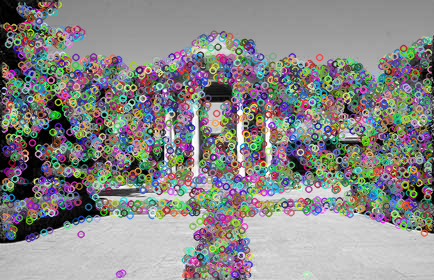
\includegraphics[height=55mm]{10-2-sift-cmp-1.png}}
\\ 
\small  \textbf{تصویر اصلی}  & \small \textbf{تصویر مقایسه}
\end{tabular}}
\vspace{-0.3cm}
\end{center}

\begin{center}
\makebox[\textwidth]{%
\begin{tabular}{@{}c}
\frame{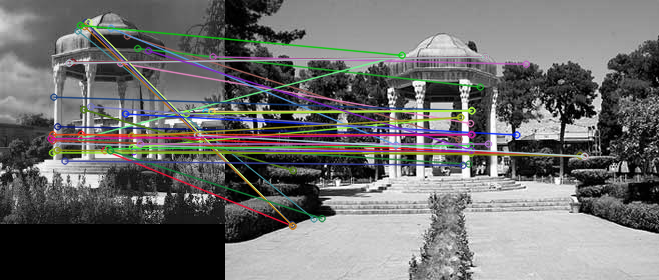
\includegraphics[height=60mm]{10-1-sift-match-1.png}} 
\\ 
\small  \textbf{نقاط منطبق با فاصله‌ی کمتر از ۸۰} 
\end{tabular}}
\end{center}

نتایج برای تصویر دوم و با پارامترهای پیش‌فرض به این شکل است:

\begin{center}
\makebox[\textwidth]{%
\begin{tabular}{@{}cc@{}}
\frame{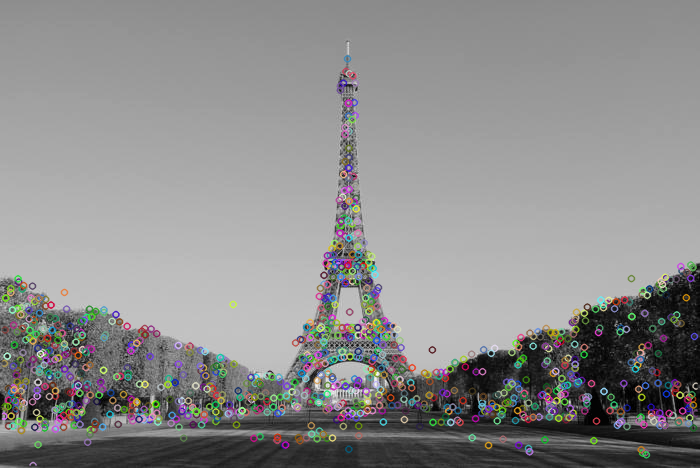
\includegraphics[height=60mm]{11-1-sift-src.png}} 
&
\frame{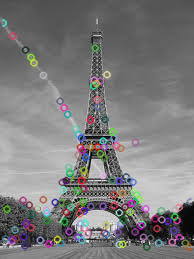
\includegraphics[height=60mm]{11-2-sift-cmp.png}}
\\ 
\small  \textbf{تصویر اصلی}  & \small \textbf{تصویر مقایسه}
\end{tabular}}
\end{center}

\begin{center}
\vspace{-0.1cm}
\makebox[\textwidth]{%
\begin{tabular}{@{}c}
\frame{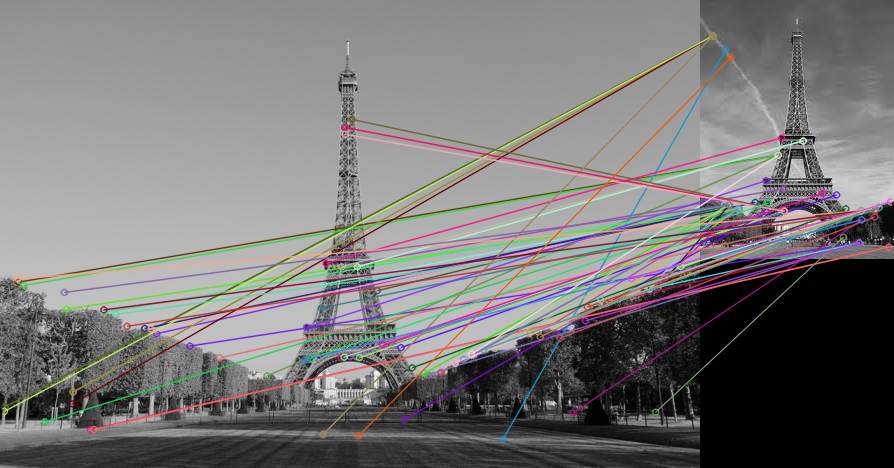
\includegraphics[height=60mm]{11-1-sift-match.png}} 
\\ 
\small  \textbf{نقاط منطبق با فاصله‌ی کمتر از ۱۰۰} 
\end{tabular}}
\vspace{-0.5cm}
\end{center}

اجرا با مقدار واریانس یک: 
\begin{center}
\vspace{-0.1cm}
\makebox[\textwidth]{%
\begin{tabular}{@{}cc@{}}
\frame{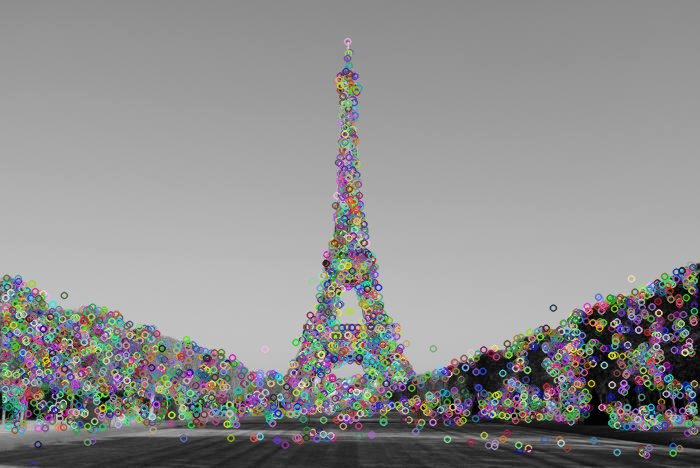
\includegraphics[height=55mm]{11-1-sift-src-1.png}} 
&
\frame{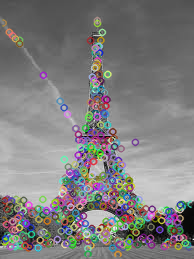
\includegraphics[height=55mm]{11-2-sift-cmp-1.png}}
\\ 
\small  \textbf{تصویر اصلی}  & \small \textbf{تصویر مقایسه}
\end{tabular}}
\end{center}

\begin{center}
\makebox[\textwidth]{%
\begin{tabular}{@{}c}
\frame{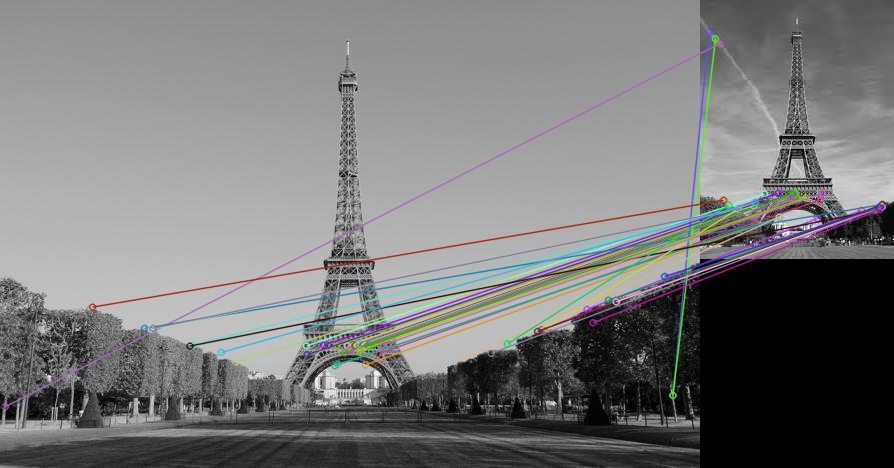
\includegraphics[height=60mm]{11-1-sift-match-1.png}} 
\\ 
\small  \textbf{نقاط منطبق با فاصله‌ی کمتر از ۱۰۰} 
\end{tabular}}
\end{center}
\vspace{1cm}


\subsection{\lr{SURF}}
\textbf{پرسش: }
الگوریتم \lr{SURF} یکی از چندین الگوریتمی است که بر پایه الگوریتم \lr{SIFT} نوشته شده است. در دو پاراگراف و به طور خلاصه تفاوت دو روش و بهبودهای بدست آمده را شرح دهید.

\textbf{پاسخ: } 

در \lr{SIFT} از تفاضل‌‌ گاسی\LTRfootnote{ DoG - Difference of Gaussian} استفاده می‌شود در صورتی که در \lr{SURF} از ماتریس هسی\LTRfootnote{ Hessian Matrix} استفاده می‌شود که دقت و کارآیی بیشتری دارد. در \lr{SIFT} هرمی از رزولوشن‌های تصویر می‌سازد و سپس فیلترهای گاسی با افزایش سیگما (واریانس) را به آن‌ها اعمال می‌کند و سپس تفاضل آن‌ها را محاسبه می‌نماید. این عمل معادل لاپلاس گرفتن از تابع گاسی و اعمال آن به تصویر است. در نهایت با محاسبه‌ی جهت گرادیان در اطراف نقطه‌ی کلیدی پیدا شده در مرحله‌ی قبل، به آرایه‌ای از هیستوگرام‌ها (برای نمونه
\( 4 \times 4 \)
)
 برای نواحی مختلف اطراف تصویر می‌رسیم که هر کدام، برای نمونه، ۸ جهت نماینده‌ی بازه‌هایی از تمامی جهات را شامل می‌شوند و به این شکل، یک توصیف ۱۲۸ بعدی از نقطه‌ی کلیدی خواهیم داشت که نسبت به تبدیلات هندسی و تغیرات شدت روشنایی و نویز، تا حد بسیار زیادی مقاوم است.

اما در \lr{SURF} چنین نیست. در اصل در \lr{SURF} از موجک‌های دو بعدی هار\LTRfootnote{ 2D Haar wavelet} و از تصویرِ انتگرال\LTRfootnote{ Integral Image} استفاده می‌شود. 
در \lr{SURF} با استفاده از یک تقریب خطی از لکه‌یاب هسی\LTRfootnote{ Hessian blob detector} که توسط تصویر انتگرال محاسبه می‌شود، سرعت بسیار بیشتر می‌شود و در اطراف این نقطه‌ی مهم، از جمع موجک‌های هار استفاده می‌کند تا نقطه را توصیف کند و این نیز به وسیله‌ی تصویر انتگرال قابل محاسبه‌ است. از آن‌جا که این روش به نوعی از \lr{Look up Table} استفاده می‌کند بار پردازشی آن کاهش یافته است. این روش تعداد نقاط کمتری پیدا می‌کند ولی سرعت آن به مراتب از \lr{SIFT} بیشتر است.

\section{\lr{HOG}}

\subsection{تشخیص انسان}

\textbf{پرسش: }
یکی از کاربردهای اصلی روش \lr{HOG} تشخیص افراد پیاده در تصاویر است. این روش در \lr{opencv} پیاده‌سازی شده و آماده استفاده است. در مجموعه داده موجود در سایت دانشگاه \lr{MIT} به آدرس

\url{http://cbcl.mit.edu/cbcl/software-datasets/PedestrianData.html}

 با استفاده از \lr{HOG} پیاده ها را بیابید.

\textbf{پاسخ: } 
پیاده‌سازی ضمیمه شده‌است.
\vspace{0.5cm}

\textbf{پرسش: }
نتایج اعمال روش را با تصاویر نمونه از موارد موفقیت و شکست و همچنین با درصد بیان کنید.

\textbf{پاسخ: } 

در این روش نمونه‌های موفق بسیاری دیده شد که در زیر آورده شده‌است: 
\begin{center}
\vspace{-0.1cm}
\makebox[\textwidth]{%
\begin{tabular}{cccc}
\multicolumn{4}{c}{}\\
\frame{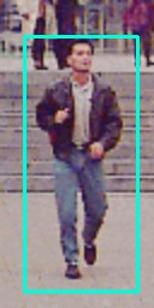
\includegraphics[height=55mm]{suc-1.png}} 
&
\frame{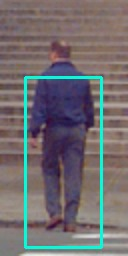
\includegraphics[height=55mm]{suc-4.png}}
& 
\frame{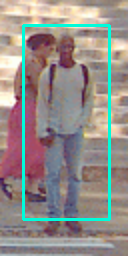
\includegraphics[height=55mm]{suc-10.png}} 
&
\frame{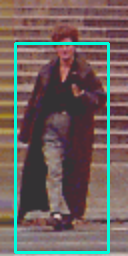
\includegraphics[height=55mm]{suc-7.png}}
\\
\end{tabular}}
\end{center}
\vspace{1cm}

مواردی از شکست نیز آورده شده‌است: 

\begin{center}
\vspace{-0.1cm}
\makebox[\textwidth]{%
\begin{tabular}{cccc}
\multicolumn{4}{c}{}\\
\frame{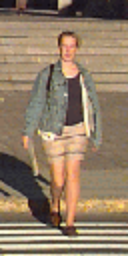
\includegraphics[height=55mm]{fail-1.png}} 
&
\frame{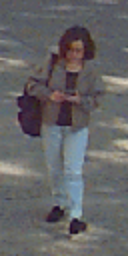
\includegraphics[height=55mm]{fail-3.png}}
& 
\frame{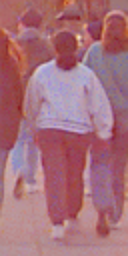
\includegraphics[height=55mm]{fail-13.png}} 
&
\frame{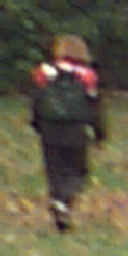
\includegraphics[height=55mm]{fail-7.png}}
\\
\end{tabular}}
\end{center}

مواردی از تشخیص اشتباه نیز آورده شده‌است: 

\begin{center}
\vspace{-0.1cm}
\makebox[\textwidth]{%
\begin{tabular}{cccc}
\multicolumn{4}{c}{}\\
\frame{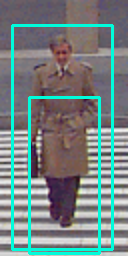
\includegraphics[height=55mm]{wro-1.png}} 
&
\frame{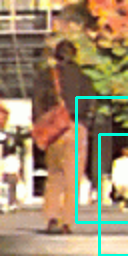
\includegraphics[height=55mm]{wro-2.png}}
& 
\frame{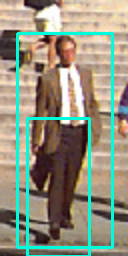
\includegraphics[height=55mm]{wro-3.png}} 
&
\frame{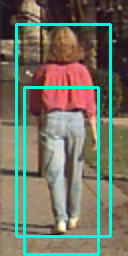
\includegraphics[height=55mm]{wro-4.png}}
\\
\end{tabular}}
\end{center}
\vspace{0.5cm}

در کل دقت تشخیص را حدود ۹۴ درصد به‌دست آوردیم: 

\begin{center}
\vspace{-0.1cm}
\makebox[\textwidth]{%
\begin{tabular}{c}
\frame{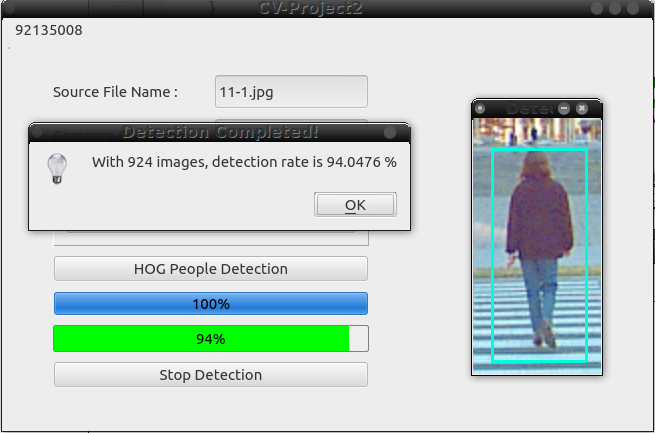
\includegraphics[height=85mm]{screenshot24.png}} 
\end{tabular}}
\end{center}
\vspace{1cm}

به نظر می‌رسد با پایین آمدن رزولوشن یا اثر لرزش، و نیز وجود سایه و یا شلوغی بیش از حد، این روش خطای زیادی دارد. 

\vspace{1cm}
\subsection{بهبود \lr{HOG}}
\textbf{پرسش: }
چه مزایا و معایبی در این روش می بینید؟ تحقیقات زیادی به افزایش کارایی روش \lr{HOG} پرداخته و تاکنون الگوریتم های متعددی بر این پایه ارائه شده اند. یکی از روش های تعمیم یافته از روش \lr{HOG} را به طور خلاصه توضیح دهید.


\textbf{پاسخ: } 

در یکی از کارهای کاملا به‌روز در این زمینه\cite{hogimp}، از روشی نوین برای تنظیم پارامترهای این الگوریتم استفاده‌ شده‌است. به این ترتیب که از یک \lr{LSVM}\LTRfootnote{ Latent SVM} استفاده شده‌است و اندازه‌ی پنجره‌ی تشخیص، اندازه‌ی سلول و نسبت ظاهری\LTRfootnote{ Aspect Ratio} را تنظیم می‌کند. در این الگوریتم نمونه‌های آموزشی بهینه می‌شوند تا ماشین بردار پشتیبان بهترین مقادیر برای پارامترهای یادشده برای الگوریتم را یاد گیرد و از یک روش منفی‌کاوی سخت\LTRfootnote{ Hard negative mining method} برای جلوگیری از تشخیص‌های اشتباه استفاده شده‌است. با توجه به این نکات، این الگوریتم یک ماشین بردار پشتیبان را برای کاربرد تشخیص انسان بهینه نموده‌است. 

\newpage




%دستوری برای به حالت عادی درآمدن اندازه فونت‌ها 


\small
%ایجاد «مراجع»


\begin{thebibliography}{99}

\begin{LTRitems}

\resetlatinfont

\bibitem{sift}
Lowe, David G. "Distinctive image features from scale-invariant keypoints." International journal of computer vision 60, no. 2 (2004): 91-110.

\bibitem{hogimp}
Gao, Chao, Fengcai Qiao, Xin Zhang, and Hui Wang. "An Improved HOG Based Pedestrian Detector." In Foundations and Practical Applications of Cognitive Systems and Information Processing, pp. 577-590. Springer Berlin Heidelberg, 2014.

\end{LTRitems}

\end{thebibliography}


\end{document} 
